%
%\subsection{Understanding Spark Application Concepts}\label{subsec:understanding-spark-application-concepts}
%
%\begin{frame}
%    \frametitle{Understanding Spark Application Concepts}
%    \begin{itemize}
%        \item \textbf{Job}: A parallel computation consisting of multiple tasks that gets spawned in response
%        to a Spark action (e.g., save(), collect()).
%        \item \textbf{Stage}: Each job gets divided into smaller sets of tasks called stages that depend on each
%        other.
%        \item \textbf{Task}: A single unit of work or execution that will be sent to a Spark executor.
%    \end{itemize}
%\end{frame}
%
%\begin{frame}
%    \frametitle{Spark Jobs}
%    \begin{figure}
%        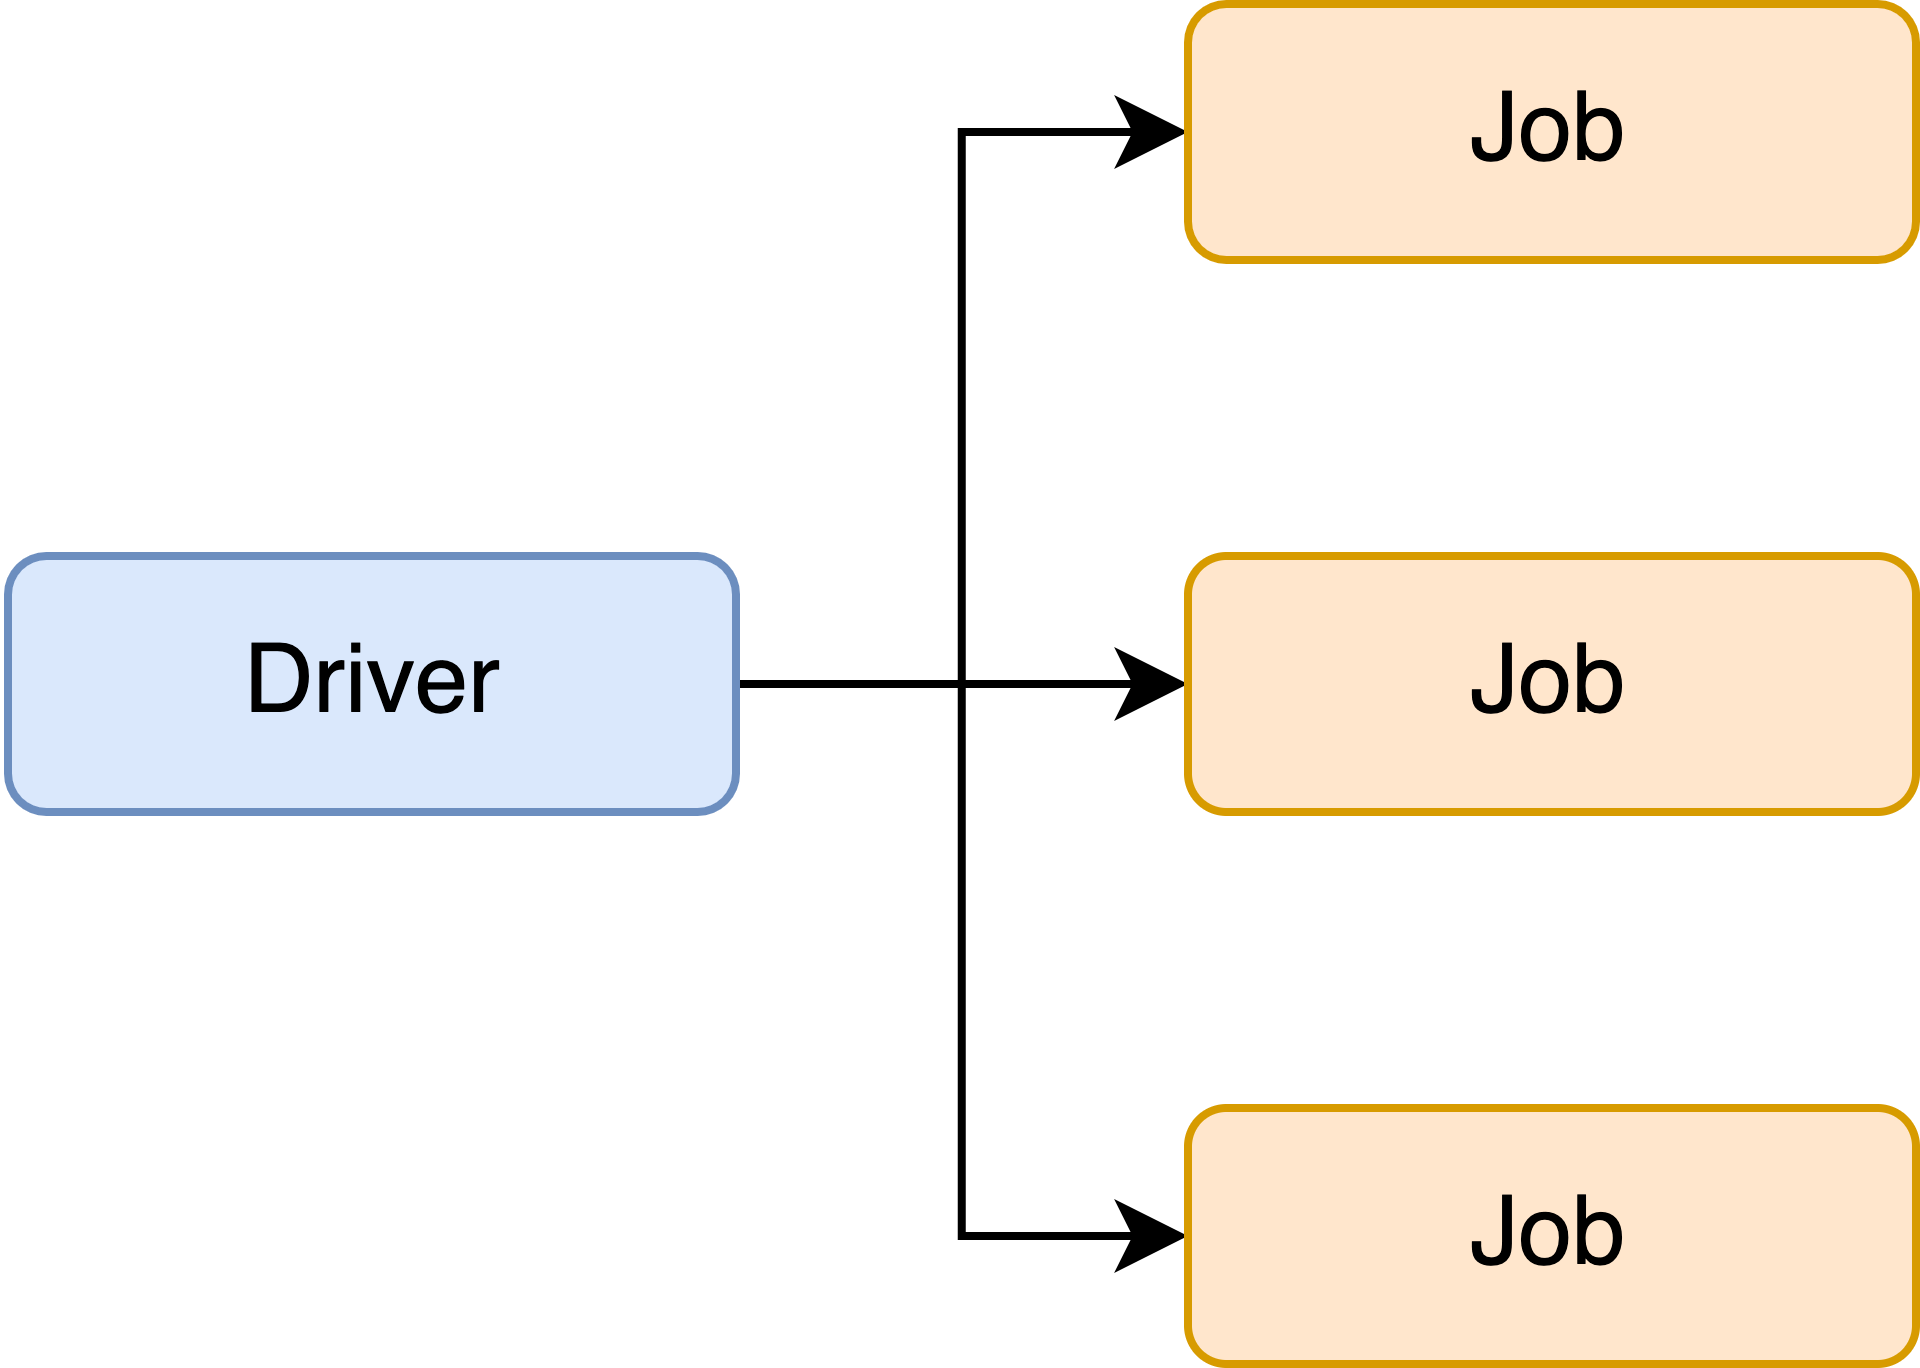
\includegraphics[width=\textwidth,height=.7\textheight,keepaspectratio]{./Figures/chapter-04/spark_job}
%        \caption{Spark driver creating one or more Spark jobs.}\label{fig:spark_job}
%    \end{figure}
%\end{frame}
%
%\begin{frame}
%    \frametitle{Spark Stages}
%    \begin{figure}
%        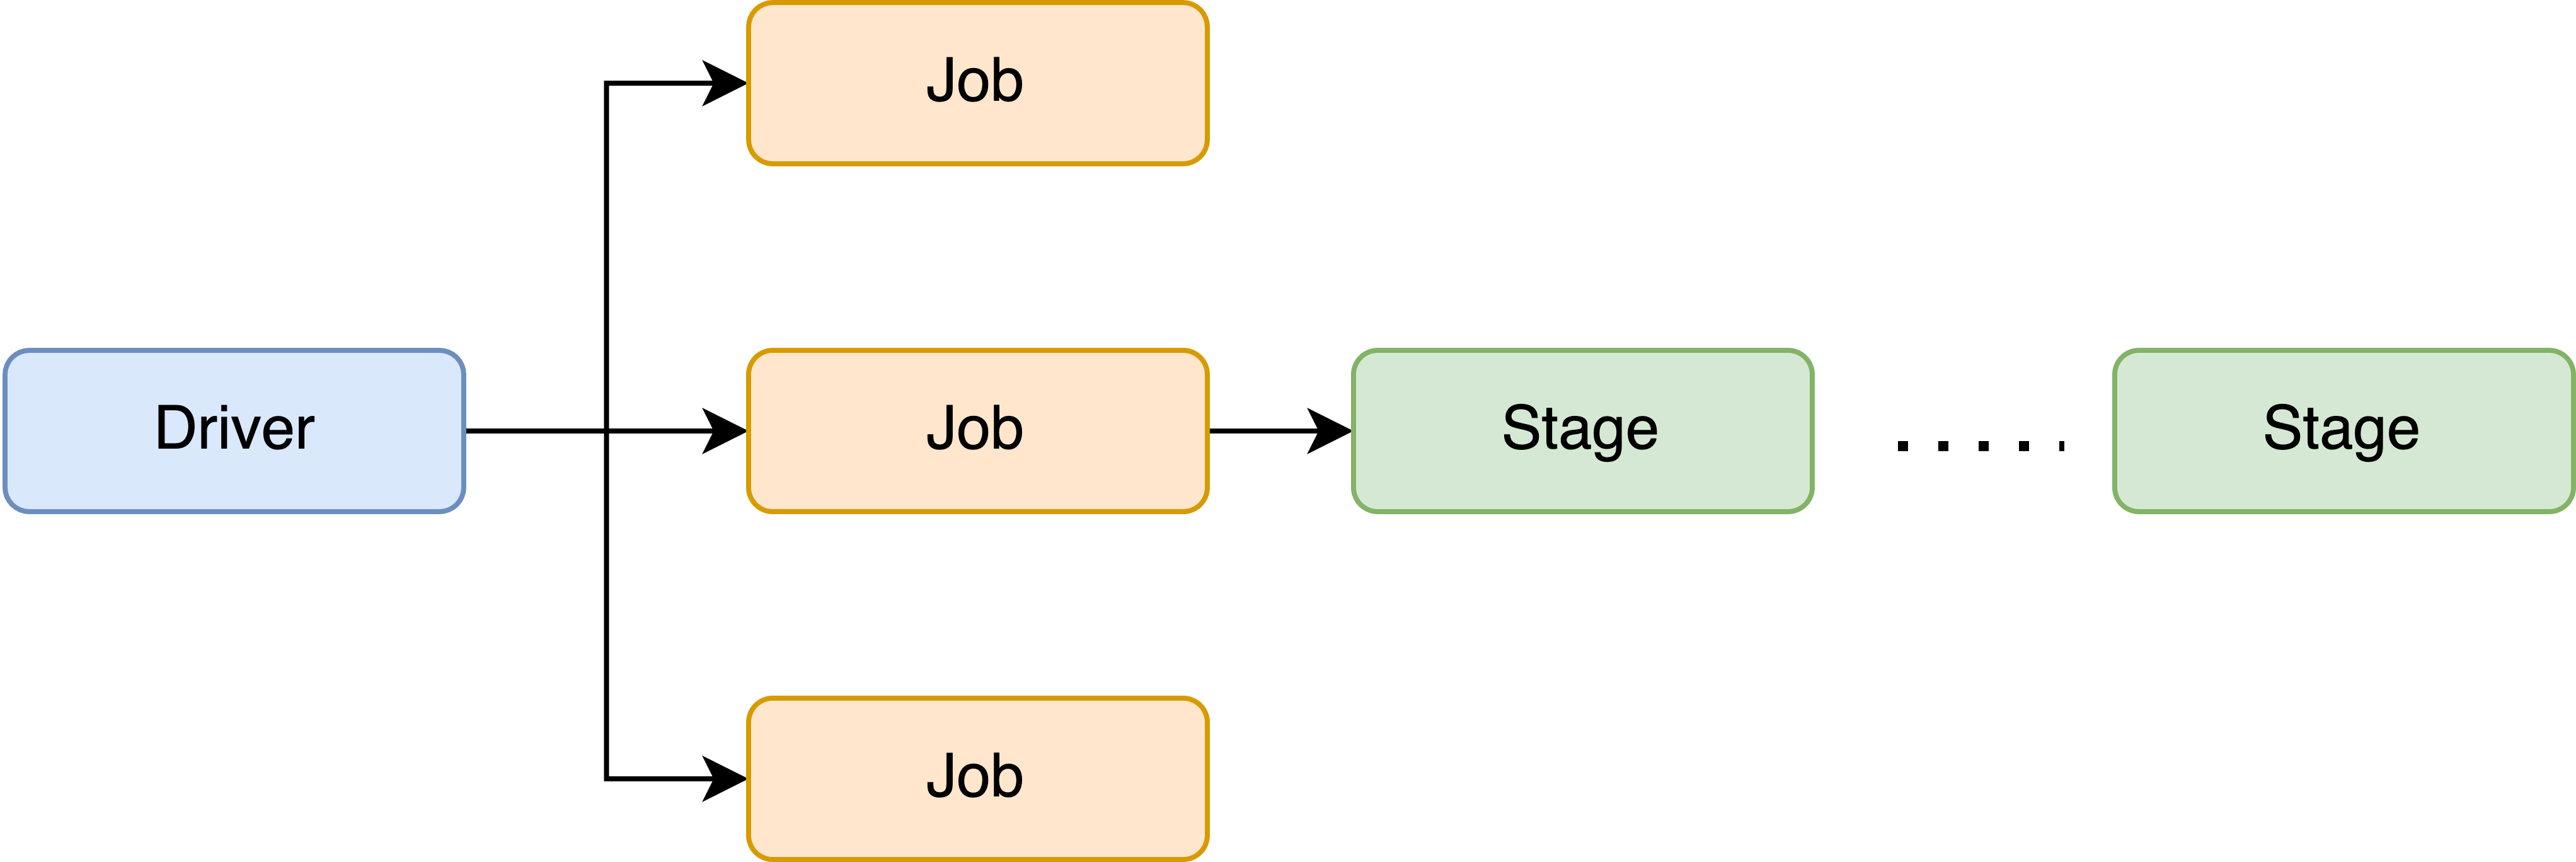
\includegraphics[width=\textwidth,height=.65\textheight,keepaspectratio]{./Figures/chapter-04/Spark_Stages}
%        \caption{Spark job creating one or more stages}\label{fig:spark_stages}
%    \end{figure}
%\end{frame}
%
%\begin{frame}
%    \frametitle{Spark Stages}
%    \begin{figure}
%        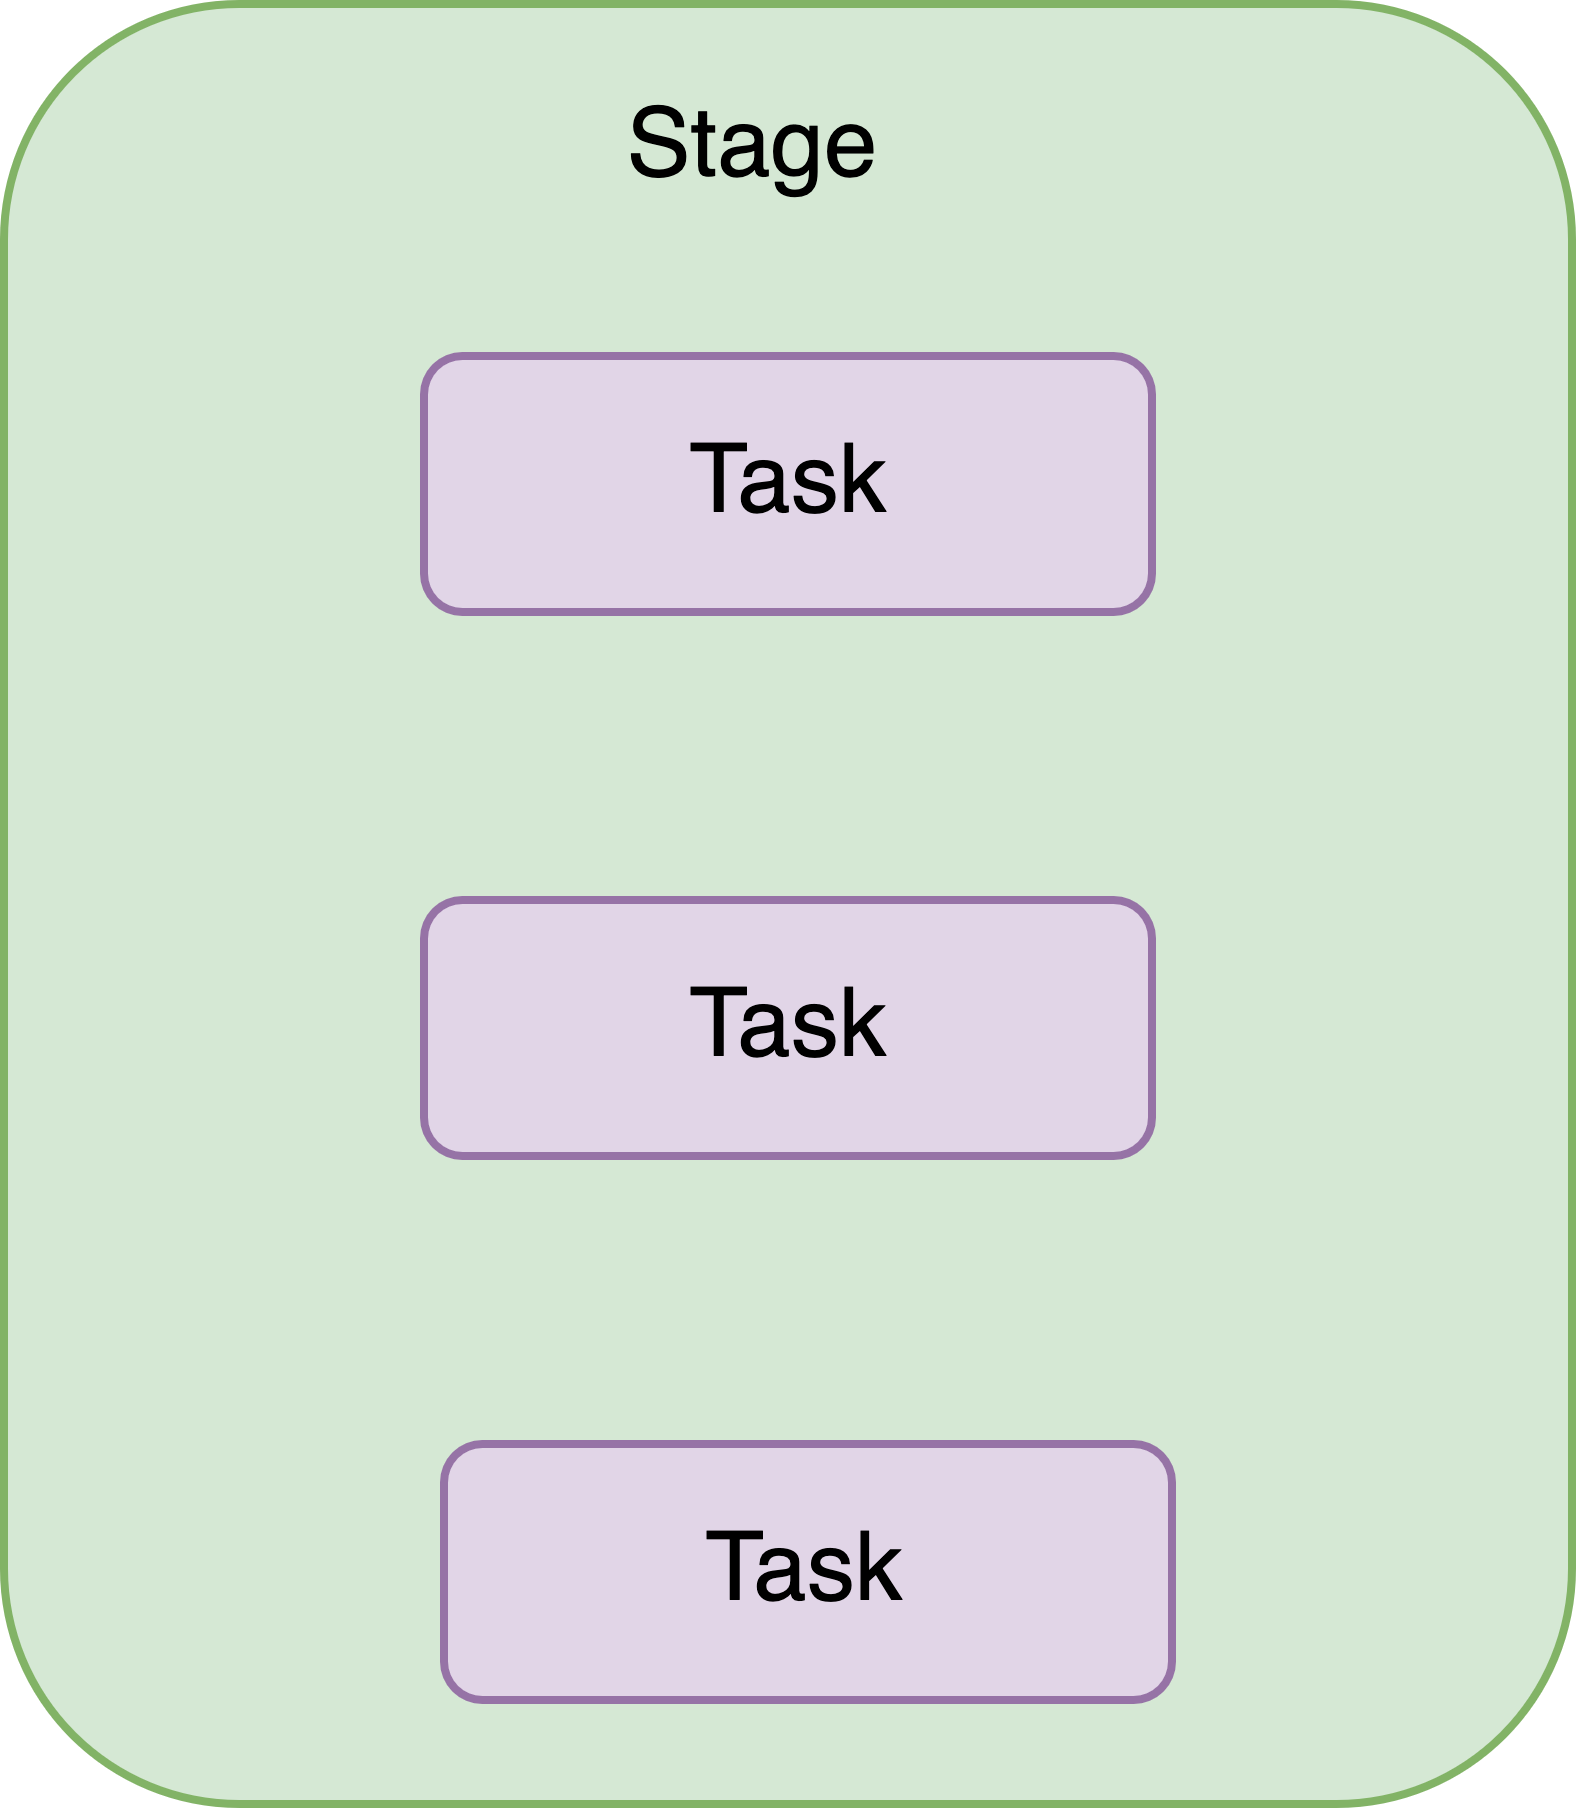
\includegraphics[width=\textwidth,height=.7\textheight,keepaspectratio]{./Figures/chapter-04/Spark_Stage}
%        \caption{Spark stage creating one or more tasks to be distributed to executors}\label{fig:spark_stage}
%    \end{figure}
%\end{frame}

%\begin{frame}
%    \frametitle{Spark Tasks}
%    \begin{figure}
%        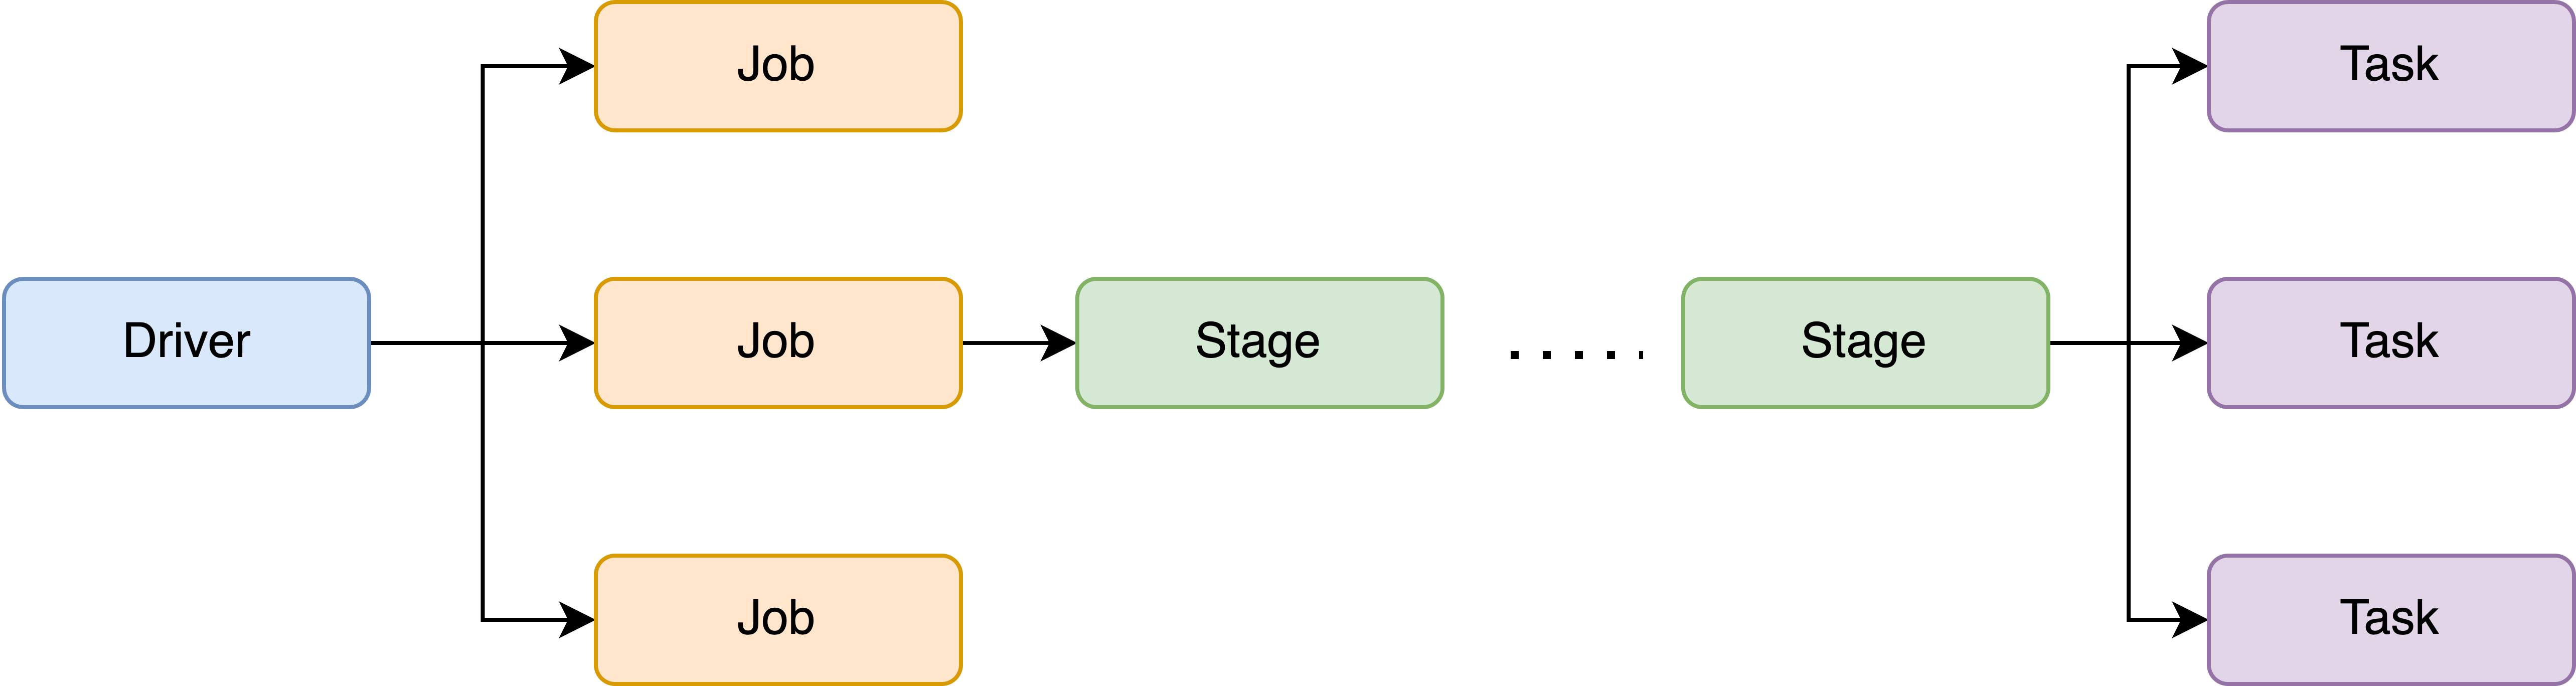
\includegraphics[width=\textwidth,height=.7\textheight,keepaspectratio]{./Figures/chapter-04/Spark_tasks}
%        \caption{Spark stage creating one or more tasks to be distributed to executors}\label{fig:Spark_tasks}
%    \end{figure}
%\end{frame}
%
%\subsection{Running Word Count \& Aggregation using Spark}\label{subsec:running-word-count-&-aggregation-using-spark}
%
%\subsection{Spark Application Life Cycle}\label{subsec:spark-application-life-cycle}
%%%%% Later
%\begin{frame}
%    \frametitle{The Life Cycle of a Spark Application (Inside Spark)}
%    \begin{itemize}
%        \item The Life Cycle of a Spark Application (Inside Spark)
%    \end{itemize}
%\end{frame}
%\begin{frame}
%    \frametitle{The Life Cycle of a Spark Application (Outside Spark)}
%    \begin{itemize}
%        \item The Life Cycle of a Spark Application (Outside Spark)
%    \end{itemize}
%\end{frame}
%\begin{frame}
%    \frametitle{The Life Cycle of a Spark Application (Inside Spark)}
%    \begin{itemize}
%        \item The Life Cycle of a Spark Application (Inside Spark)
%    \end{itemize}
%\end{frame}
%
%\begin{frame}
%    \frametitle{ADVANCED: SPARK DRIVER INTERNAL SCHEDULER}
%    \begin{itemize}
%        \item GOING DEEPER INTO SPARK DRIVER.
%        \item CAN WE OPTIMIZE SPARK DRIVER WORKLOAD?
%    \end{itemize}
%\end{frame}
%%%%%%%%%%%%%%%%%%%%%%%%%%%%%%%%%%%%%%%%%%%%%%%%%%%%%%%
%
%\subsection{Further Readings and Assignment}
